\chapter{Introdução}\label{Cap:Introduction}
	
% \section{Motivation}

O tráfego de aplicativos de realidade virtual (VR) e realidade aumentada (AR) deverá crescer consideravelmente nos próximos anos~\cite{Cisco2020}. Certamente, o streaming de vídeos esféricos, ou, vídeos 360$^\circ$ é um dos principais fatores desse crescimento, especialmente com a proliferação de head-mounted displays (HMD) acessíveis, como Meta Quest 3 e Apple Vision Pro, juntamente com a popularidade crescente de vídeos de $360^\circ$ em plataformas como Facebook e YouTube. No entanto, o streaming de vídeos esféricosainda enfrenta muitos desafios para operar perfeitamente e oferecer experiência de alta qualidade sob diversas condições de rede. Isso ocorre pois esse tipo de vídeo exige consideravelmente mais recursos de processamento e rede em comparação com o streaming de vídeo 2D padrão. Por esta razão vários estudos sobre esse tema foi observado nos últimos anos. 

Hoje em dia, o streaming de vídeos esféricos dependem principalmente da arquitetura de streaming de vídeo 2D. Assim, toda a esfera de vídeo precisa primeiro ser projetada em um plano usando alguma técnica de projeção (por exemplo, equirretangular ou \textit{cubemap}) antes de ser comprimida com um codificador de vídeo 2D padrão, como H.264 ou H.265. 
Para streaming, geralmente é empregado o protocolo Dynamic Adaptive Streaming over HTTP (DASH), pelo qual o servidor disponibiliza o vídeo em vários segmentos de duração fíxas, codificados em diversas qualidades/taxas de bits. No lado do cliente do aplicativo pode solicitar os pedaços de vídeo com base em algum algoritmo de taxa de bits adaptativo (ABR) que observa a largura de banda disponível e solicita a qualidade adequada. 

No entanto, ao contrário dos vídeos 2D, um usuário só pode visualizar uma fração de todo o vídeo devido a limitação do campo de visão humano (FOV), conforme mostrado na Figura~\ref{fig:viewport}(a). Normalmente, um HMD tem um FoV de $120^{\circ}\times90^{\circ}$, o que corresponde a apenas 16,6\% de toda a esfera~\cite{Afzal2017}. Consequentemente, recursos significativos do sistema (por exemplo, largura de banda, bateria e memória) podem ser desperdiçados se todo o vídeo esférico for transmitido (também conhecido como streaming "monolítico"), especialmente se esses vídeos forem transmitidos com definição muito alta.

\begin{figure}[htb]
\centering
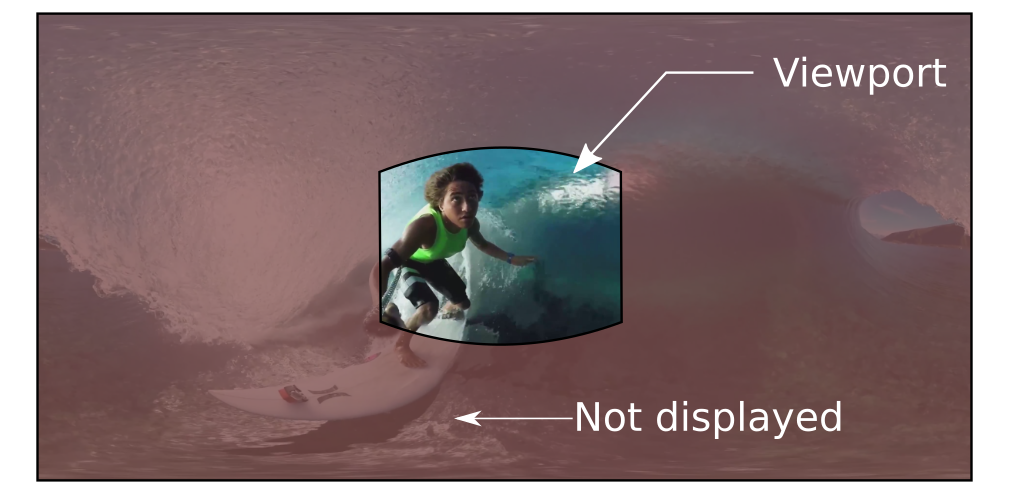
\includegraphics[width=0.49\columnwidth]{fig/viewport1.png} \hfill
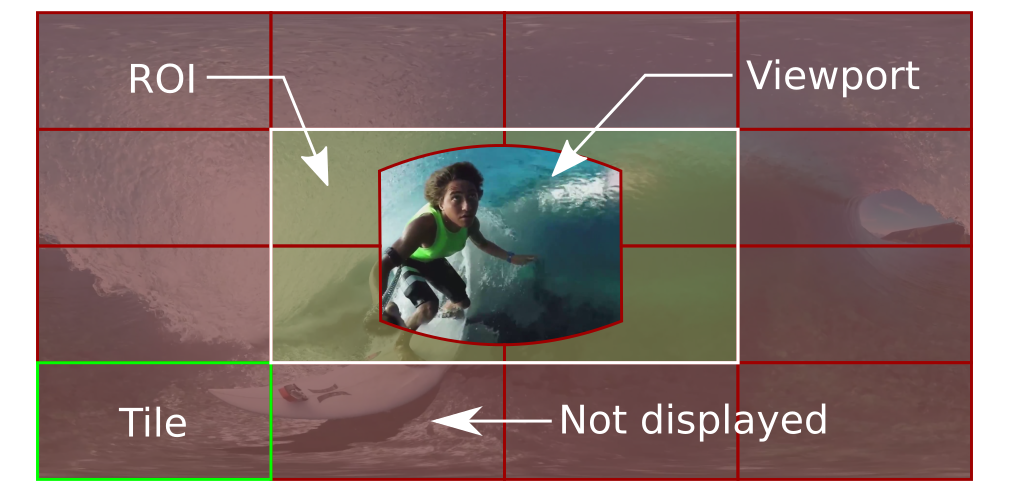
\includegraphics[width=0.49\columnwidth]{fig/viewport2.png} \\
\caption{(a) Viewport em um streaming monolítico: desperdício ao requisitar pixels não vistos (em vermelho). (b) Um vídeo ladrilhado no formato $4 \times 4$ com região de interesse (em verde) e viewport.}
\label{fig:viewport}
\end{figure}

Para economizar recursos, vários trabalhos~\cite{Zare2016, Graf2017, Hosseini2017, Xiao2018} adotaram uma abordagem adaptativa à janela de visualização para o streaming de vídeos de $360^\circ$. Neste caso, a projeção do vídeo é segmentada espacialmente em ladrilhos independentes, de modo que o cliente possa solicitar apenas aqueles que abrangem as viewports previstas para os próximos segundos. A figura~\ref{fig:viewport}(b) apresenta esta abordagem utilizando um padrão de ladrilho $4 \times 4$ com um ROI e uma janela de visualização correspondente.

Nessa linha, Qian et al.~\cite{Qian2018} propuseram uma solução baseada em ladrilhos voltada para dispositivos móveis comuns. O algoritmo ABR proposto otimiza o número e o tamanho (ou seja, a qualidade) dos blocos a serem solicitados com base em uma restrição que leva em consideração o diversas características do vídeo, estimados a partir de médias de amostra avaliadas em tempo de execução, entre outros parâmetros. Consequentemente, a restrição sobre a qual uma decisão ótima é tomada assume que um único valor “típico” do tempo de decodificação do bloco é válido para todos os tamanhos pesquisáveis de blocos (isto é, qualidades). Tal suposição pode gerar problemas de ocupação do \textit{buffer} que podem levar a interrupções indesejáveis na reprodução. Portanto, embora a solução do sistema dos autores ofereça um excelente desempenho, acreditamos que seu trabalho também lançou alguma luz sobre a necessidade de investigar mais detalhadamente as características dos ladrilhos. Na verdade, o status de ocupação do \textit{buffer} é fundamental no projeto de algoritmos ABR~\cite{Huang2014}, e entender seu comportamento por meio de filas ou teoria de controle provou ser uma ferramenta poderosa~\cite{Huang2014,Yin2015,Spiteri2016,Yadav2017} . Para ajudar nisso, é necessário algum conhecimento estatístico do comportamento do tráfego de entrada/saída do \textit{buffer} de um cliente. Embora considerável atenção na literatura tenha sido dada à caracterização da largura de banda da rede em vídeos esféricos com ladrilhos, nenhum trabalho anterior tratou da caracterização do modelo de transmissão de vídeo que correlacione a qualidade percebida pelo cliente com a qualidade das projeções codificadas no servidor.


% \section{objectives}

% \subsection{General Objectives}

% \subsection{Specific Objectives}

% \section{Related Works}

% \section{Contribuição}

Neste trabalho apresentamos a modelagem de um sistema de transmissão de vídeo 360 graus codificado com HEVC, considerando diferentes tipos de segmentação espacial e qualidade em streaming de vídeo sob demanda com DASH. Estimamos a da função de densidade com base em uma série de experimentos realizados em um conjunto de vídeos de $360^\circ$ com diferentes características espaciais, temporais e observacionais. Além disso, investigamos até que ponto o tempo de decodificação do bloco está correlacionado com a taxa de bits do bloco (no nível do bloco), para que o streaming de vídeo baseado em DASH possa possibilitar o uso de tal informação para otimizar a transmissão de vídeo. Esses dados podem ser usados para emular a reprodução de uma sessão de vídeo 360 para que possamos analisar o desempenho dos algoritmos ABR.

% \section{Metodologia}

A metodologia deste trabalho envolve o cálculo de métricas estatísticas de sistemas de transmissão de vídeo, que serão utilizadas para a avaliação do desempenho de streaming de vídeo em 360 graus para diferentes algoritmos de adaptação de taxa de bits (ABR). As métricas consideradas incluem tempo de decodificação, taxa de transmissão e qualidade medida em MSE e outras métricas de erro próprias para vídeo esféricos. O modelo é utilizado para emular um usuário assistindo a uma seção de vídeo, capturando traços de rede para avaliação de desempenho e otimizando a qualidade da transmissão de forma eficiente.

% \section{Organização}

O restante deste estudo está organizado da seguinte forma: No Capítulo 2, é realizada uma revisão do estado da arte para sistemas de transmissão de vídeo de 360 graus com vídeo segmentado baseado em ladrilhos, considerando mecanismos de seleção de blocos, previsão de janela de visualização e bancos de dados disponíveis. O capítulo 3 concentra-se na modelagem dos objetos e métricas considerados em sistemas de transmissão. O capítulo 4 relata as análises de diferentes cenários e, por fim, no capítulo 5 são apresentadas as conclusões do trabalho desenvolvido e as propostas de trabalhos futuros para a continuação desta pesquisa.
